This section summarizes how the experiments were conducted and their results.

\subsection{Methodology} \label{subsec:methodology}
Experiments are performed using the script \verb|jacobirun.sh|, as better explained in sub-section~\ref{subsec:runningexperiments}.
The script runs sequential, thread and FastFlow versions both on the Xeon CPU and Xeon Phi co-processor.
If on the Xeon CPU The number of workers for parallel versions goes from $1$ to $16$, otherwise it ranges from $1$ to $240$ (to match the number of threads of each processor).
$N$, instead, assumes values of $5000$, $10000$, $15000$, and $30000$. Sadly bigger values of $N$ quickly filled up the memory of the co-processor, hence they were not included in the analysis.
All the tests of the FastFlow implementation use a grain size of $10$.

\subsection{Results and remarks} \label{subsec:results}
Each of the graphs in this section reports experimental results in terms of efficiency, scalability, and speedup of each experiment described above.
\begin{figure}
	\centering
	\begin{subfigure}[b]{0.3\linewidth}
		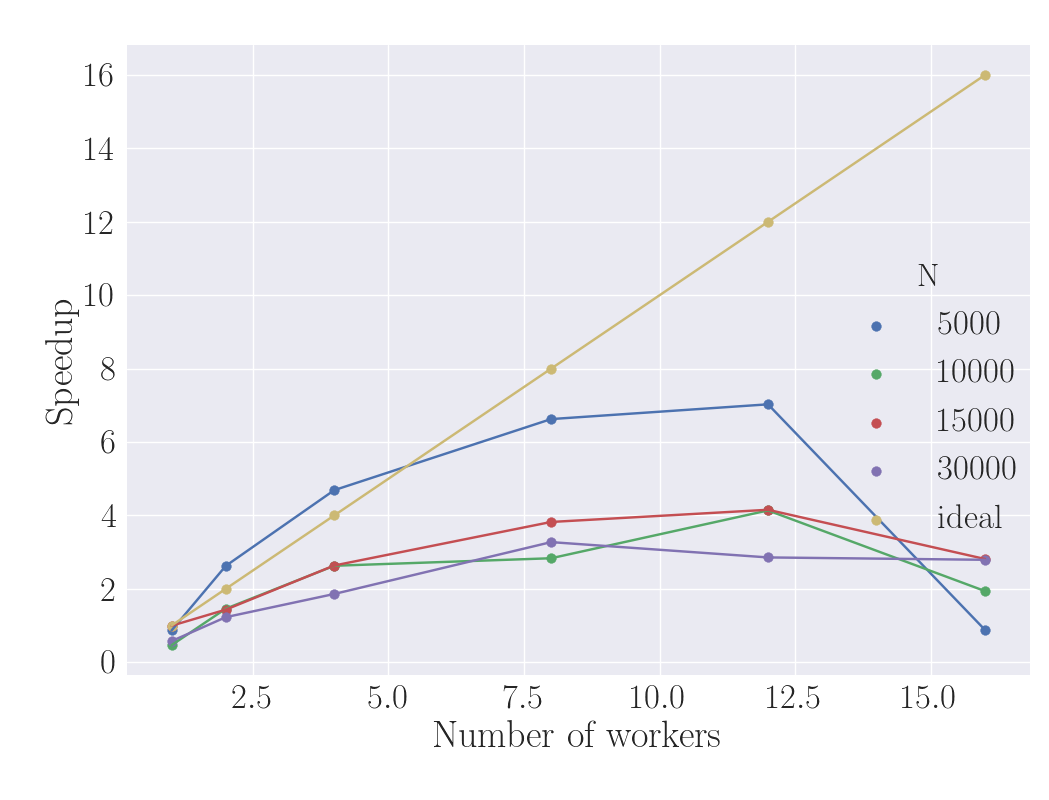
\includegraphics[width=\linewidth]{../graphs/graph_ff_host_s}
		\caption{Speedup graph.}
		\label{fig:ff_host_s}
	\end{subfigure}
	\begin{subfigure}[b]{0.3\linewidth}
		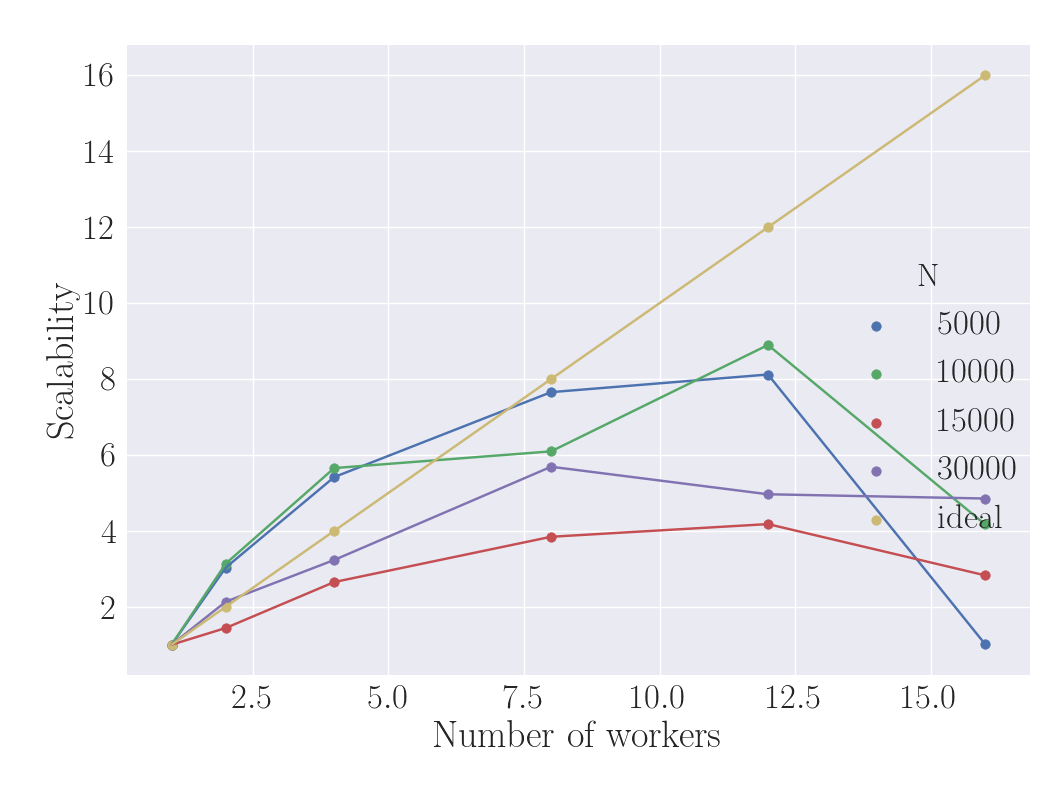
\includegraphics[width=\linewidth]{../graphs/graph_ff_host_scalab}
		\caption{Scalability graph}
		\label{fig:ff_host_scalab}
	\end{subfigure}
	\begin{subfigure}[b]{0.3\linewidth}
		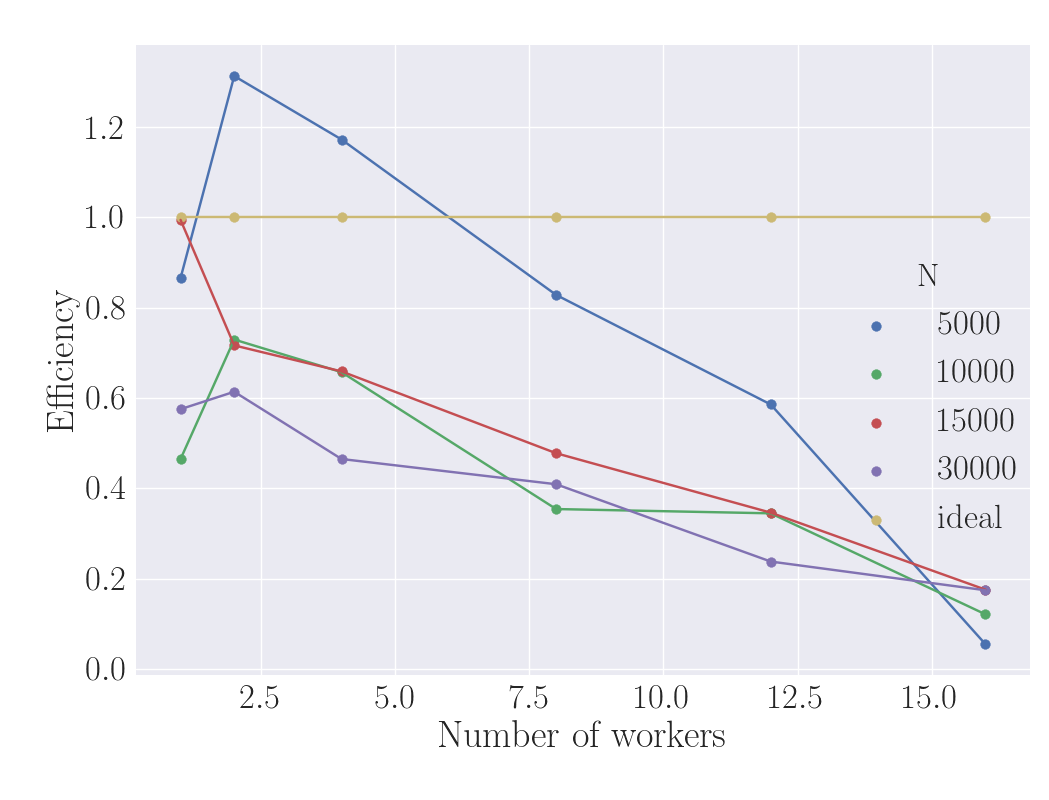
\includegraphics[width=\linewidth]{../graphs/graph_ff_host_eff}
		\caption{Efficiency graph}
		\label{fig:ff_host_eff}
	\end{subfigure}
	\caption{Graphs of different performance measures for $N \in \{5000, 10000, 15000, 30000\}$ on the Xeon CPU using FastFlow}
	\label{fig:ff_host}
\end{figure}
\begin{figure}
	\centering
	\begin{subfigure}[b]{0.3\textwidth}
		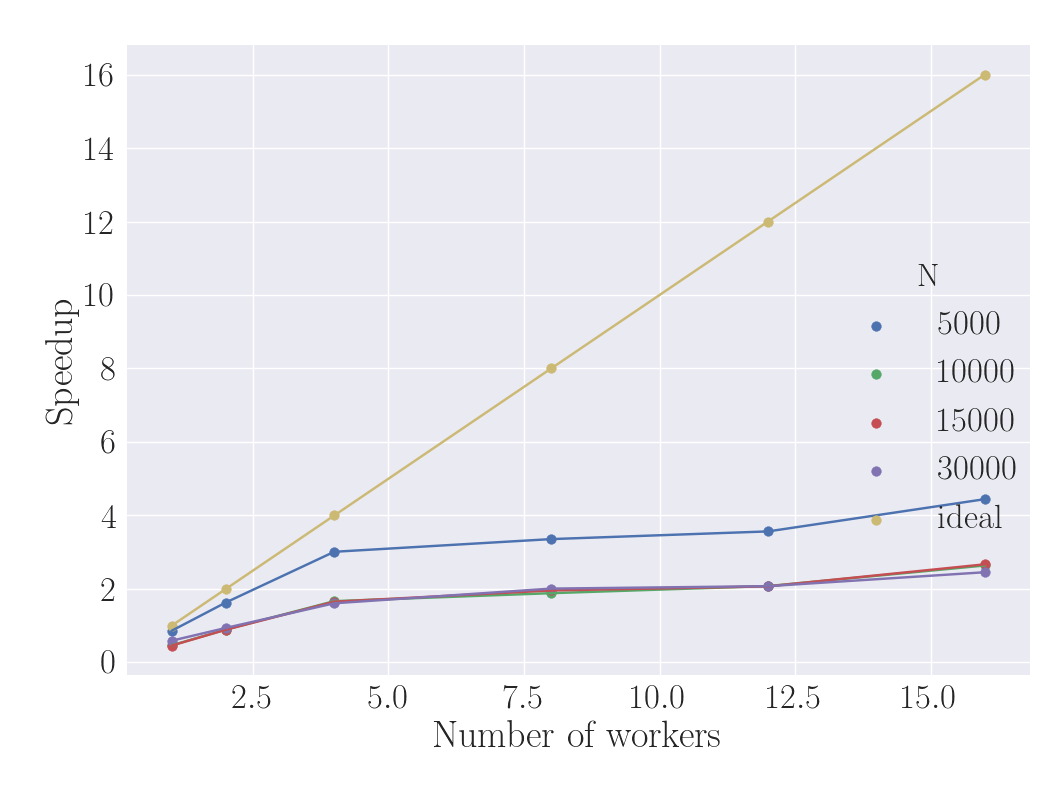
\includegraphics[width=\textwidth]{../graphs/graph_th_host_s}
		\caption{Speedup graph.}
		\label{fig:th_host_s}
	\end{subfigure}
	\begin{subfigure}[b]{0.3\textwidth}
		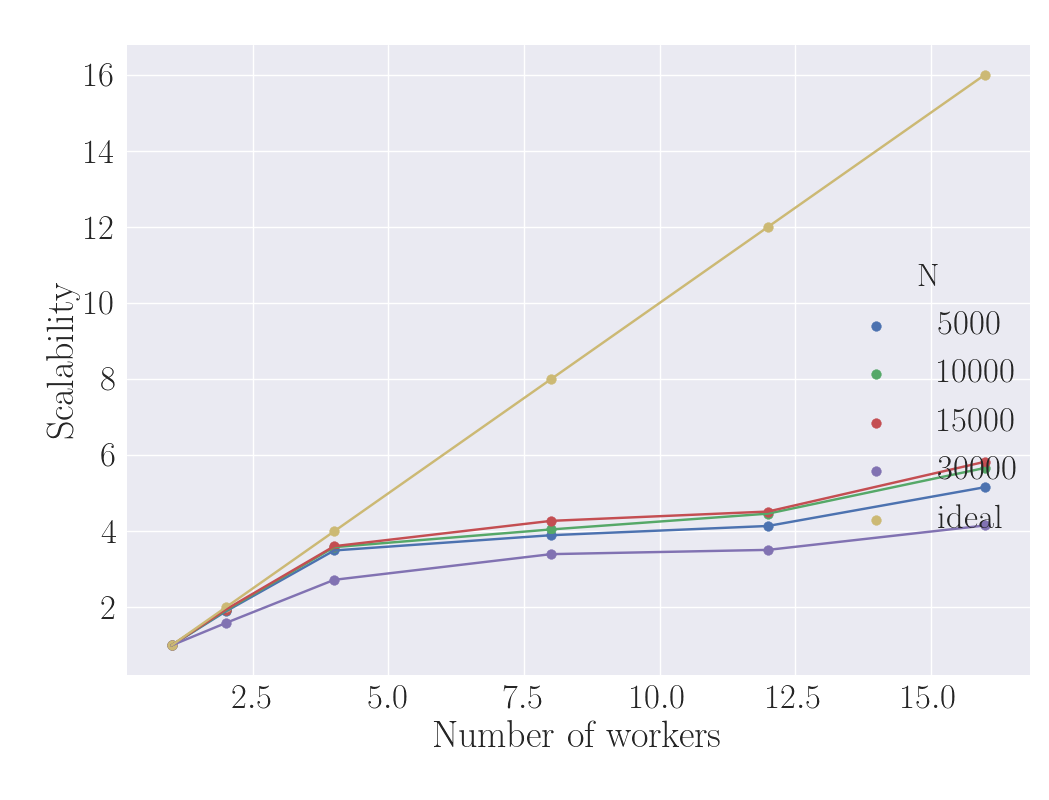
\includegraphics[width=\textwidth]{../graphs/graph_th_host_scalab}
		\caption{Scalability graph}
		\label{fig:th_host_scalab}
	\end{subfigure}
	\begin{subfigure}[b]{0.3\textwidth}
		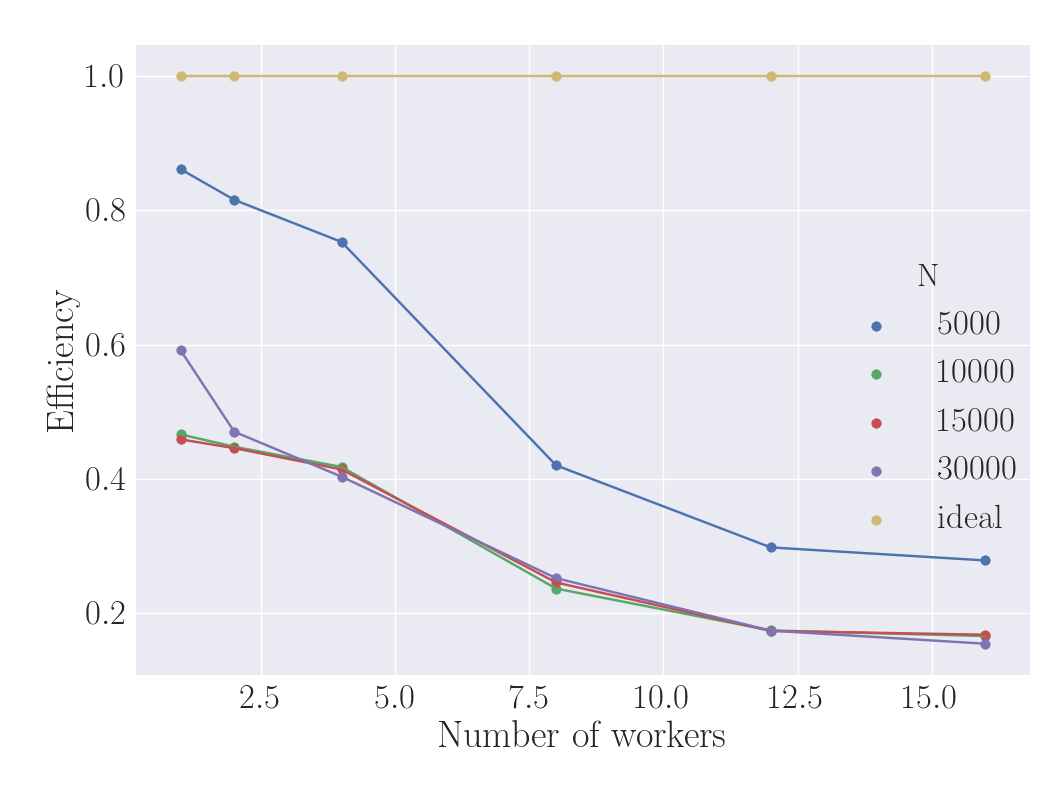
\includegraphics[width=\textwidth]{../graphs/graph_th_host_eff}
		\caption{Efficiency graph}
		\label{fig:th_host_eff}
	\end{subfigure}
	\caption{Graphs of different performance measures for $N \in \{5000, 10000, 15000, 30000\}$ on the Xeon CPU using C++11 threads}
	\label{fig:th_host}
\end{figure}
Figure~\ref{fig:ff_host} and Figure~\ref{fig:th_host} respectively report the results of the execution of the FastFlow and C++11 thread implementation on the Xeon CPU.
It is interesting to see that none of the measured metrics adhere to the ideal curve, especially for bigger $N$s.
Smaller $N$s lead to better performance metrics, probably this is partly due to the time spent in barrier and in the setup of the workers and partly due to the time spent by the processor in performing cache coherence.
\begin{figure}
	\centering
	\begin{subfigure}[b]{0.3\textwidth}
		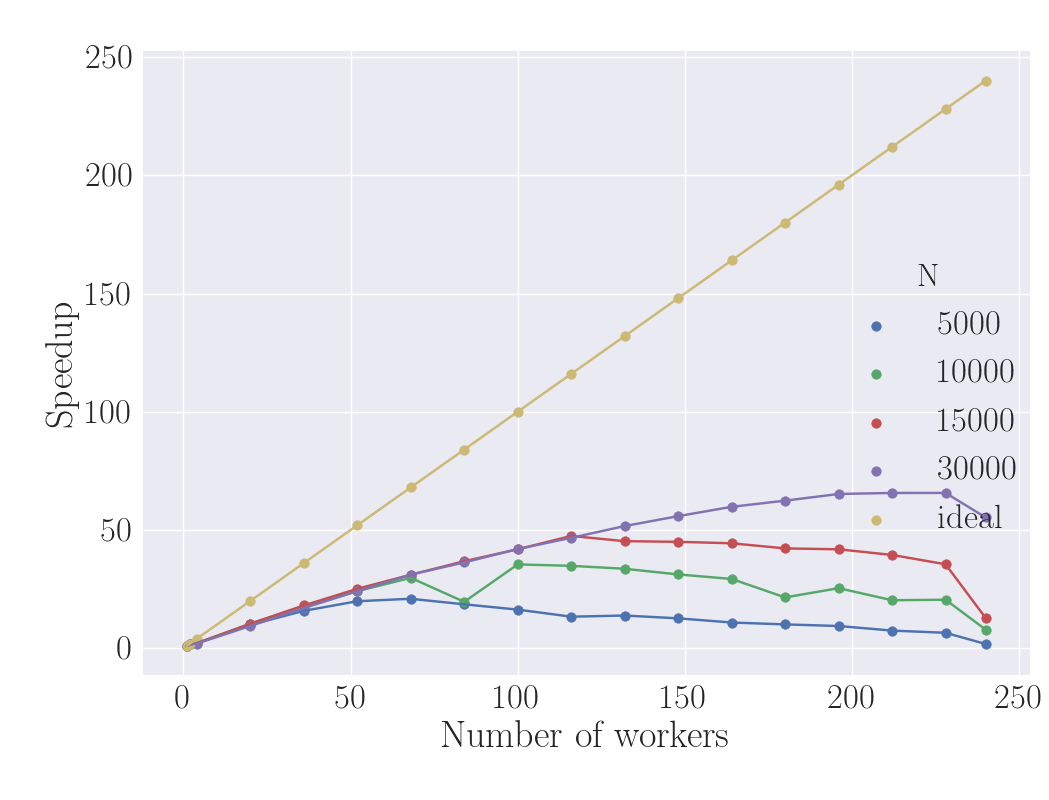
\includegraphics[width=\textwidth]{../graphs/graph_ff_mic_s}
		\caption{Speedup graph.}
		\label{fig:ff_mic_s}
	\end{subfigure}
	\begin{subfigure}[b]{0.3\textwidth}
		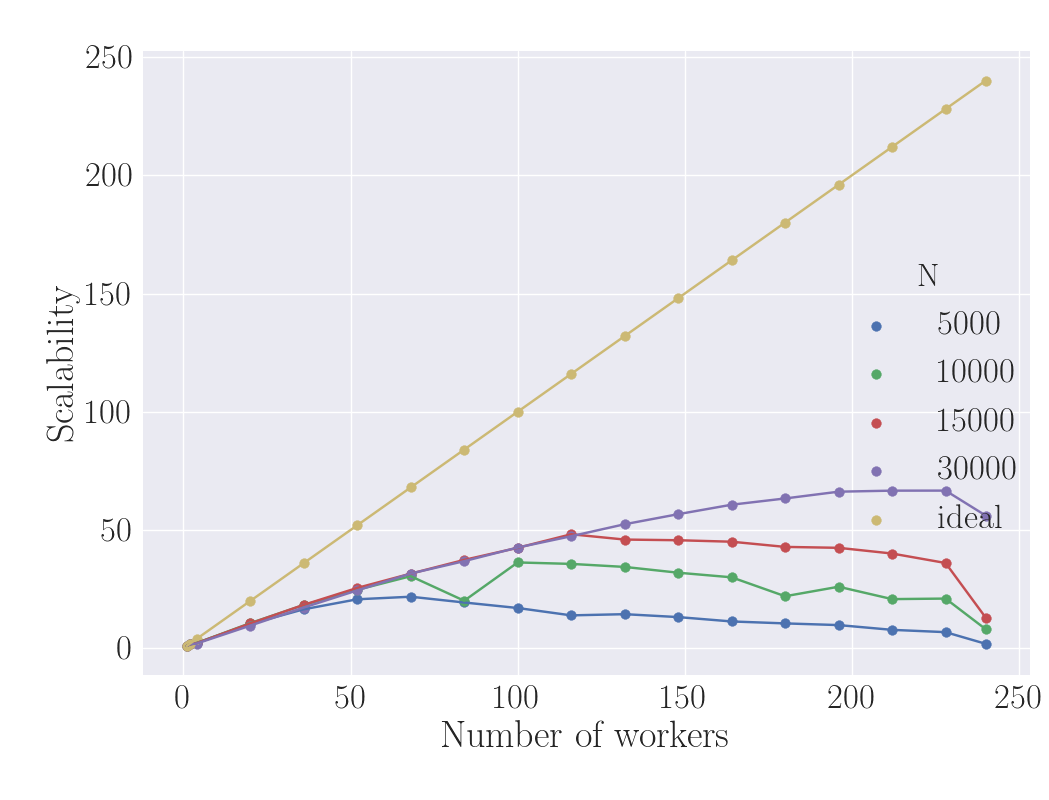
\includegraphics[width=\textwidth]{../graphs/graph_ff_mic_scalab}
		\caption{Scalability graph}
		\label{fig:ff_mic_scalab}
	\end{subfigure}
	\begin{subfigure}[b]{0.3\textwidth}
		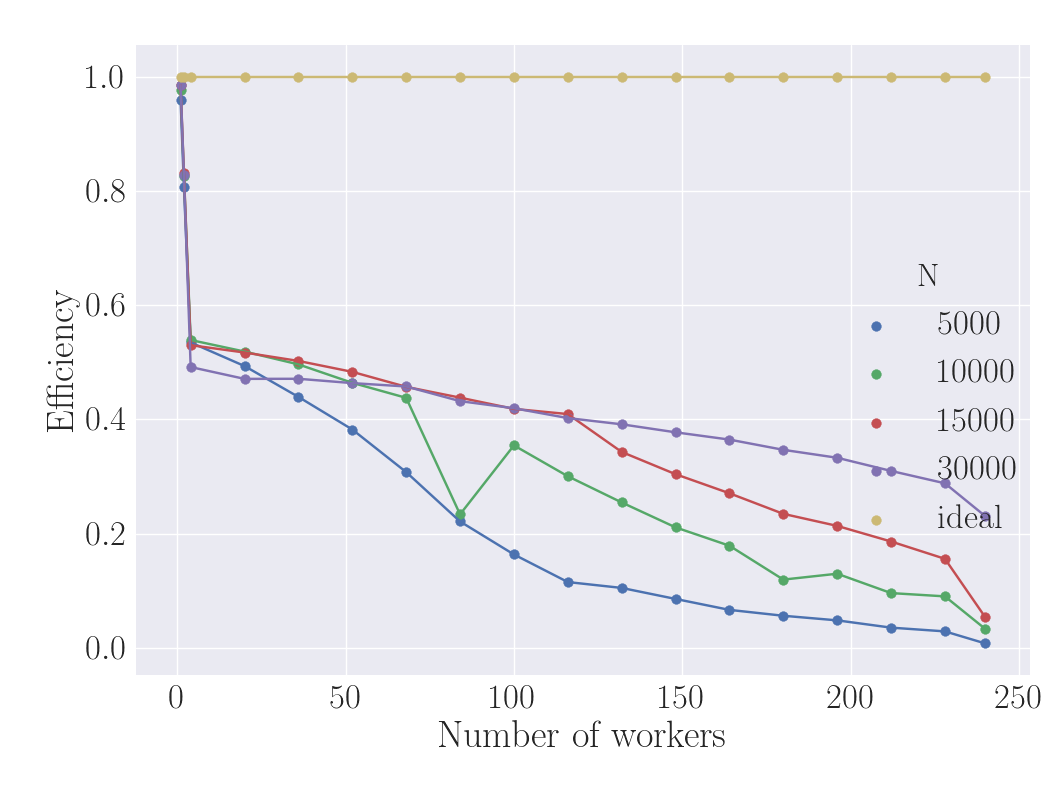
\includegraphics[width=\textwidth]{../graphs/graph_ff_mic_eff}
		\caption{Efficiency graph}
		\label{fig:ff_mic_eff}
	\end{subfigure}
	\caption{Graphs of different performance measures for $N \in \{5000, 10000, 15000, 30000\}$ on the Xeon Phi co-processor using FastFlow}
	\label{fig:ff_mic}
\end{figure}
\begin{figure}
	\centering
	\begin{subfigure}[b]{0.3\textwidth}
		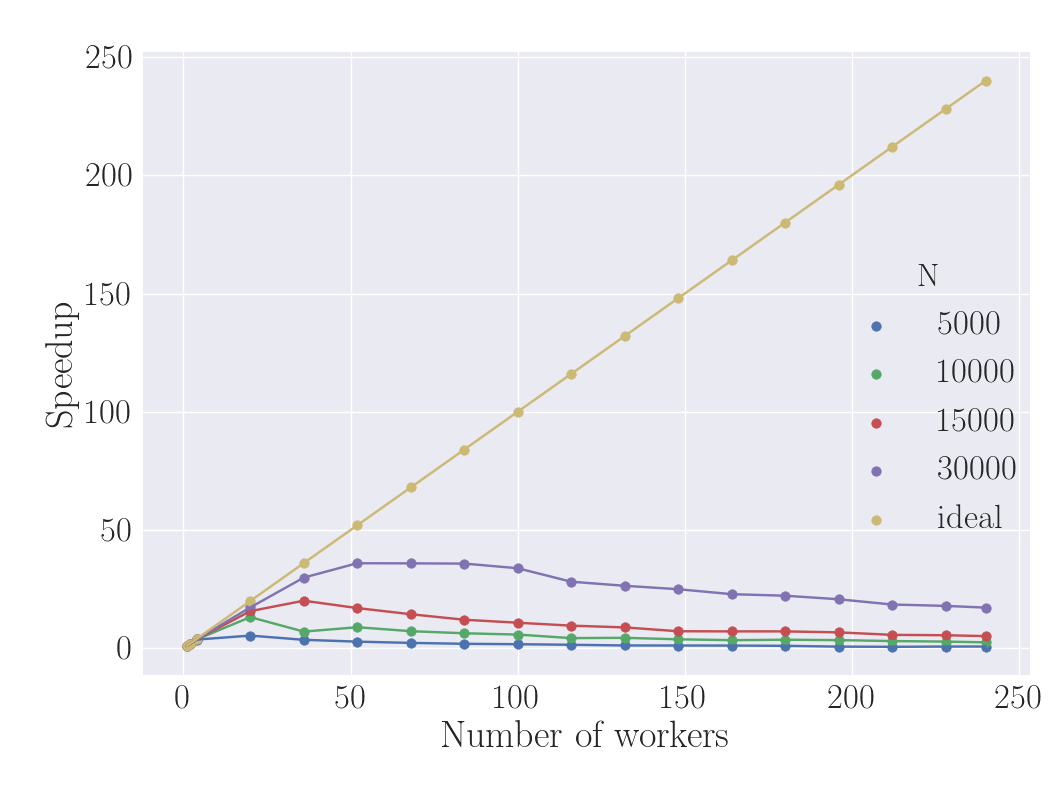
\includegraphics[width=\textwidth]{../graphs/graph_th_mic_s}
		\caption{Speedup graph.}
		\label{fig:th_mic_s}
	\end{subfigure}
	\begin{subfigure}[b]{0.3\textwidth}
		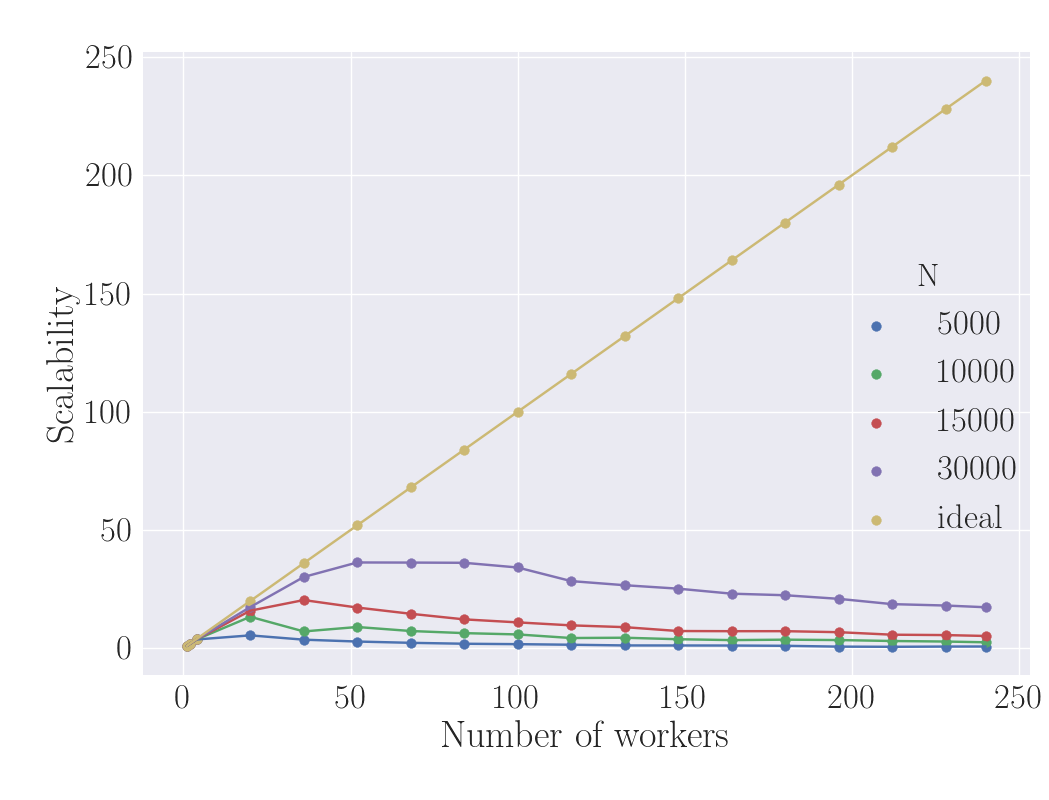
\includegraphics[width=\textwidth]{../graphs/graph_th_mic_scalab}
		\caption{Scalability graph}
		\label{fig:th_mic_scalab}
	\end{subfigure}
	\begin{subfigure}[b]{0.3\textwidth}
		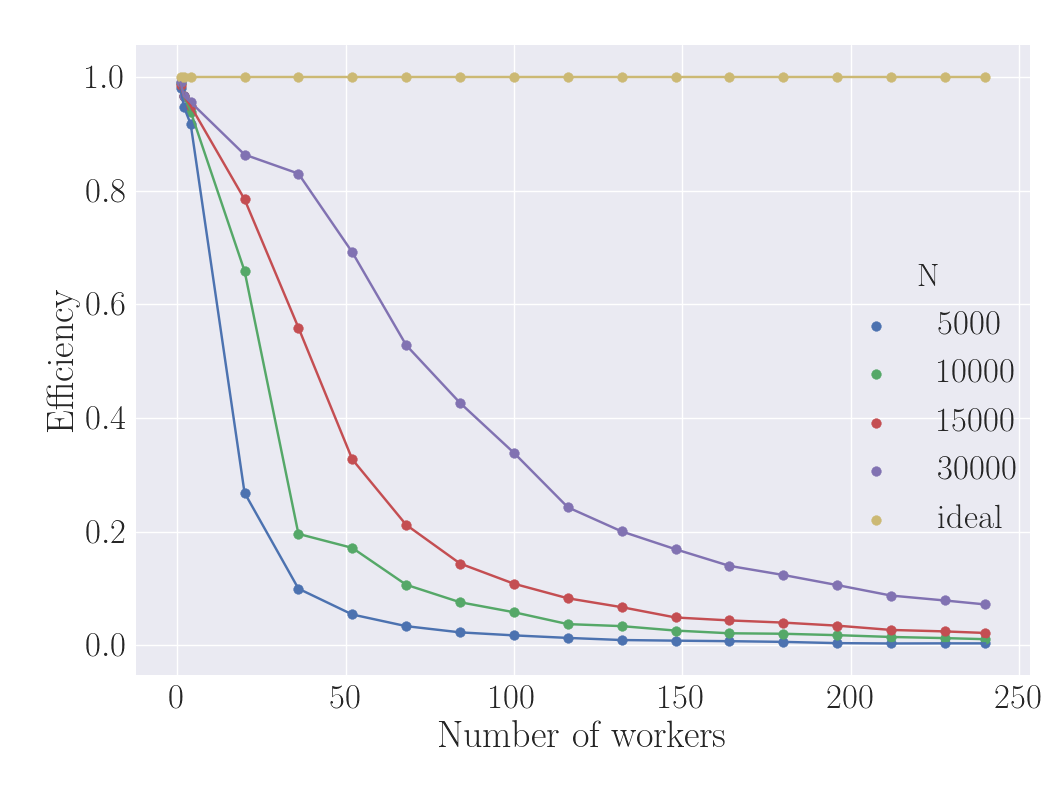
\includegraphics[width=\textwidth]{../graphs/graph_th_mic_eff}
		\caption{Efficiency graph}
		\label{fig:th_mic_eff}
	\end{subfigure}
	\caption{Graphs of different performance measures for $N \in \{5000, 10000, 15000, 30000\}$ on the Xeon Phi co-processor using C++11 threads}
	\label{fig:th_mic}
\end{figure}
Figure~\ref{fig:ff_mic} and Figure~\ref{fig:th_mic} respectively report the results of the execution of the FastFlow and C++11 thread implementation on the Xeon Phi co-processor.
As above none of the measured metrics adhere to the ideal curve.
In this case, on the other hand, bigger $N$s lead to better performance metrics since the time spent in barrier and in the setup of the workers becomes smaller w.r.t.\ effective time of computation.
In this case (up to $N = 30000$) cache coherence probably is not a bottleneck, since the cache on the Xeon Phi is bigger than the one on the Xeon CPU.
\begin{table}
	\centering
	\begin{tabular}{clcccc}  
		\toprule
		 & & \multicolumn{2}{c}{\textbf{$N = 5000$}} & \multicolumn{2}{c}{\textbf{$N = 10000$}}\\
		\midrule
		 & & \textbf{Xeon CPU} & \textbf{Xeon Phi} & \textbf{Xeon CPU} & \textbf{Xeon Phi}\\
		\cmidrule{3-6}		
		\textbf{Sequential} & Latency (\si{seconds})& $0.049155$& $0.200321$ & $0.116605$& $0.773010$\\
		\midrule
		\textbf{FastFlow} & Latency w.\ $1$ worker (\si{seconds}) & $0.064645$ & $0.209576$ & $0.256767$ & $0.799476$\\
		 & Best latency & $0.008042$ & $0.009522$ & $0.028808$ & $0.022374$\\
		 & Workers for best & $12$ & $68$ & $12$ & $116$\\
		\midrule
		\textbf{Thread} &Latency w.\ $1$ worker (\si{seconds}) & $ $ & $ $ & $ $ & $ $\\
				& Best latency & $ $ & $ $ & $ $ & $ $\\
				& Workers for best & $ $ & $ $ & $ $ & $ $ \\
				& Ratio & $ $ & $ $ & $ $ & $ $ \\
		\bottomrule
	\end{tabular}
	\caption{Best configurations in terms of minimal latency for FastFlow and Thread implementations. $N = 5000$ and $N=10000$}
	\label{tab:res0}
\end{table}
\begin{table}
	\centering
	\begin{tabular}{clcccc}  
		\toprule
		& & \multicolumn{2}{c}{\textbf{$N = 15000$}} & \multicolumn{2}{c}{\textbf{$N = 30000$}}\\
		\midrule
		& & \textbf{Xeon CPU} & \textbf{Xeon Phi} & \textbf{Xeon CPU} & \textbf{Xeon Phi}\\
		\cmidrule{3-6}		
		\textbf{Sequential} & Latency (\si{seconds}) & $0.266411$ & $1.731800$ & $1.080730$ & $6.820180$\\
		\midrule
		\textbf{FastFlow} & Latency (\si{seconds}) & $0.266411$ & $1.731800$ & $1.080730$ & $6.820180$\\
		& Best latency & $0.266411$ & $1.731800$ & $1.080730$ & $6.820180$\\
		& Workers for best & $0.266411$ & $1.731800$ & $1.080730$ & $6.820180$\\
		\midrule
		\textbf{Thread} & Latency (\si{seconds}) &  $0.266411$ & $1.731800$ & $1.080730$ & $6.820180$\\
		& Best latency & $0.266411$ & $1.731800$ & $1.080730$ & $6.820180$\\
		& Workers for best & $0.266411$ & $1.731800$ & $1.080730$ & $6.820180$\\
		& Ratio & $0.266411$ & $1.731800$ & $1.080730$ & $6.820180$\\
		\bottomrule
	\end{tabular}
	\caption{Best configurations in terms of minimal latency for FastFlow and Thread implementations. $N = 15000$ and $N=30000$}
	\label{tab:res1}
\end{table}
\alert{Table~\ref{tab:ff} shows, for each size $N$ of the system, the best configuration in terms of latency for the FastFlow implementation.
Table~\ref{tab:th} shows the same data as Table~\ref{tab:ff}, but reports also the ratio between setup/barrier time and latency (i.e.\ $({T_{barrier} + T_{setup})/T_{jacobi}$) (full data is available in folder \verb|results| as \verb|csv| file, as explained in Section~\ref{sec:guide}).}

Please note that (almost) none of the best configurations include a number of workers equal to the number of contexts, this is due to the fact that usually at least one context is used for orchestration.
